% Der Abstract richtet sich an den Spezialisten auf dem entsprechenden Gebiet
% und beschreibt daher in erster Linie die (neuen, eigenen) Ergebnisse und
% Resultate der Arbeit. Es umfasst nie mehr als eine Seite, typisch sogar nur
% etwa 200 Worte (etwa 20 Zeilen). Es sind keine Bilder zu verwenden.

\chapter*{Erklärung}\addcontentsline{toc}{chapter}{Eigenständigkeitserklärung}

Ich erkläre hiermit,
\begin{itemize}
	\item dass ich die vorliegende Arbeit selber und ohne fremde Hilfe durchgeführt habe, ausser derjenigen, welche explizit in der Aufgabenstellung erwähnt ist oder mit dem Betreuer schriftlich vereinbart wurde,
	\item dass ich sämtliche verwendeten Quellen erwähnt und gemäss gängigen wissenschaftlichen Zitierregeln korrekt angegeben habe.
	\item das ich keine durch Copyright geschützten Materialien (z.B. Bilder) in dieser Arbeit in unerlaubter Weise genutzt habe.
\end{itemize}

Ort, Datum: \\
Rapperswil, 12.06.2015

\begin{tabularx}{\textwidth}{XX}

\includegraphics[scale=1]{start/img/marcoLeutenegger} & 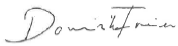
\includegraphics[scale=1]{start/img/dominikFreier} \\
Marco Leutenegger & \hspace{1cm} Dominik Freier
\end{tabularx}